\documentclass[border=10pt]{standalone}
\usepackage{tikz}
\usetikzlibrary{arrows.meta, shapes, positioning, shadows, calc}

\begin{document}
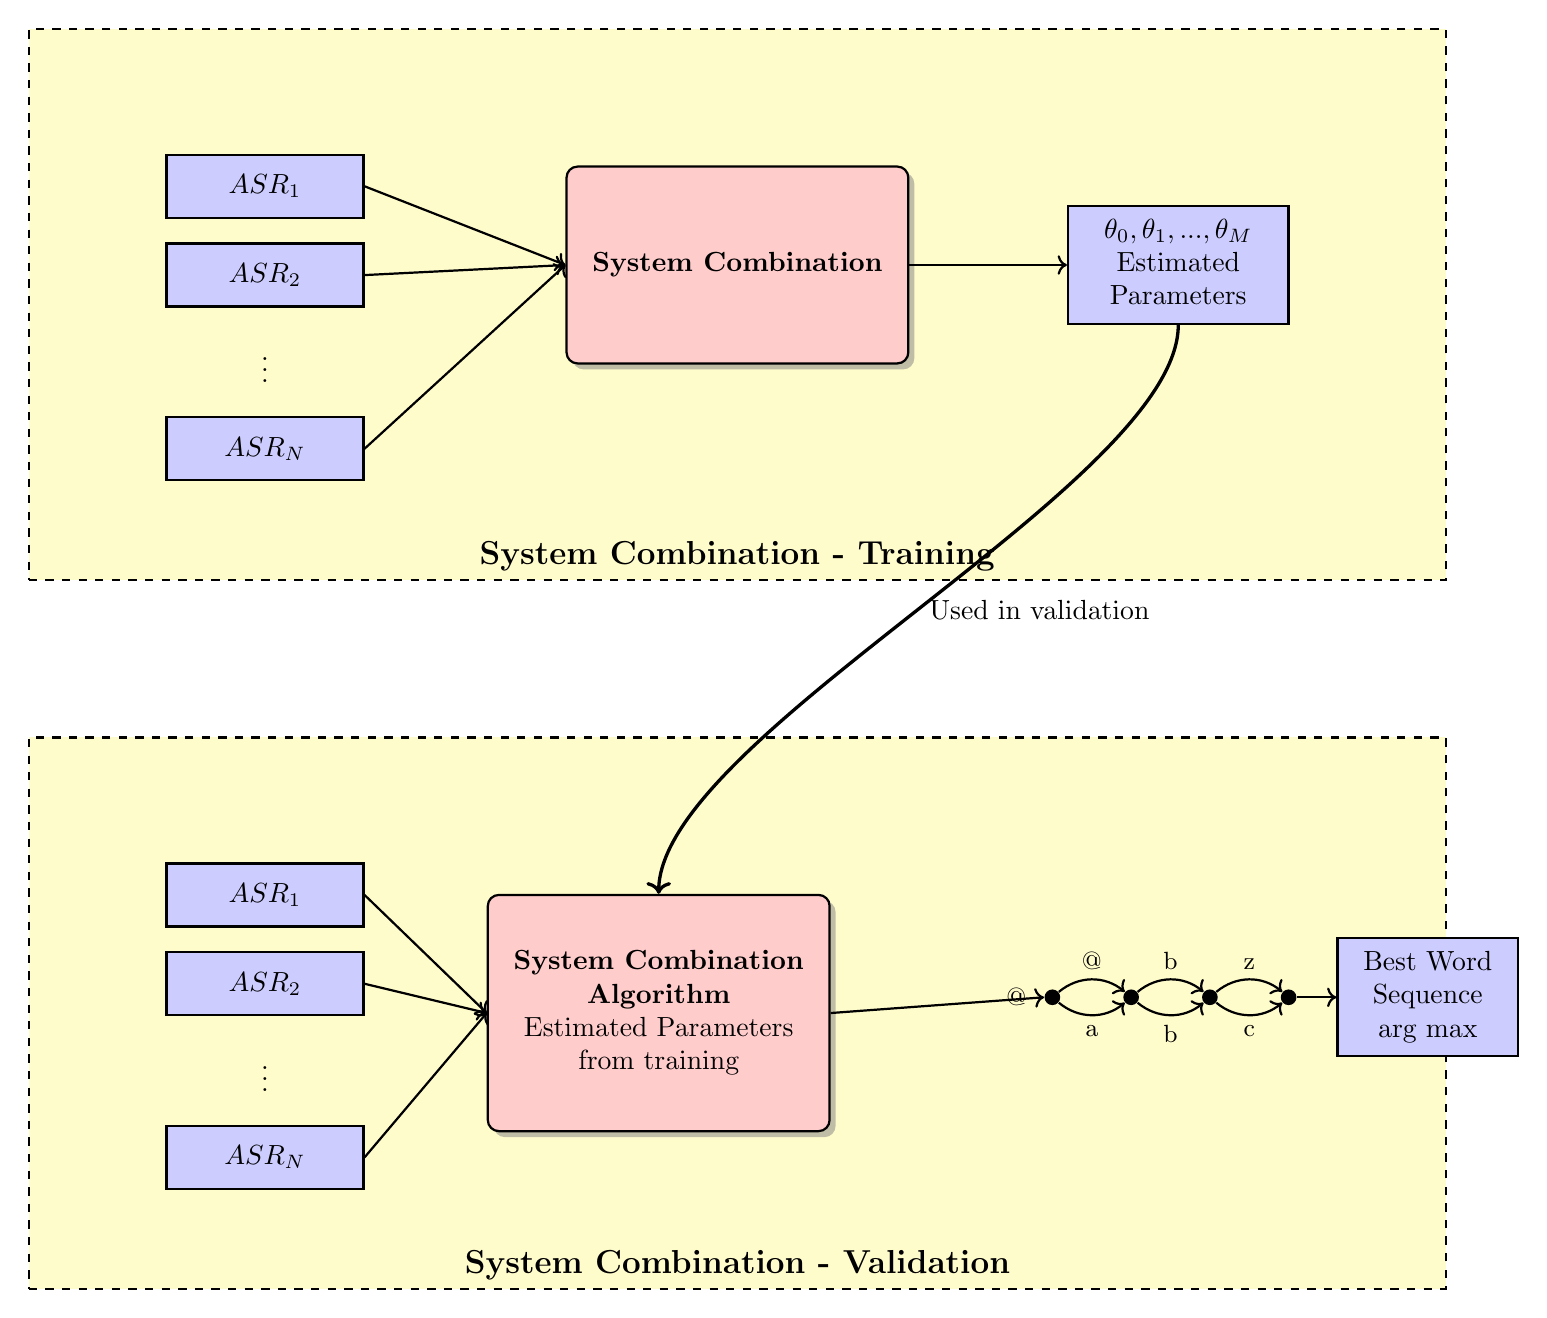
\begin{tikzpicture}[
    node distance=0.8cm,
    asrbox/.style={rectangle, draw=black, fill=blue!20, minimum width=2.5cm, minimum height=0.8cm, thick},
    combbox/.style={rectangle, rounded corners, draw=black, fill=red!20, minimum width=4cm, minimum height=2.5cm, thick, drop shadow},
    parambox/.style={rectangle, draw=black, fill=blue!20, minimum width=2.8cm, minimum height=1.5cm, thick},
    bgbox/.style={rectangle, draw=black, dashed, fill=yellow!20, thick},
    arrow/.style={->, thick}
]

% Training Section
\node[bgbox, minimum width=18cm, minimum height=7cm] (trainbg) at (0,0) {};
\node[anchor=south] at (trainbg.south) {\large\textbf{System Combination - Training}};

% ASR boxes - Training
\node[asrbox] (asr1) at (-6, 1.5) {$ASR_1$};
\node[asrbox, below=0.3cm of asr1] (asr2) {$ASR_2$};
\node[below=0.3cm of asr2] (dots1) {$\vdots$};
\node[asrbox, below=0.3cm of dots1] (asrn) {$ASR_N$};

% System Combination - Training
\node[combbox] (syscomb1) at (0, 0.5) {\begin{tabular}{c}\textbf{System Combination}\end{tabular}};

% Parameters box
\node[parambox, right=2cm of syscomb1] (params) {\begin{tabular}{c}$\theta_0, \theta_1, ..., \theta_M$\\Estimated\\Parameters\end{tabular}};

% Arrows - Training
\draw[arrow] (asr1.east) -- (syscomb1.west);
\draw[arrow] (asr2.east) -- (syscomb1.west);
\draw[arrow] (asrn.east) -- (syscomb1.west);
\draw[arrow] (syscomb1.east) -- (params.west);

% Validation Section
\node[bgbox, minimum width=18cm, minimum height=7cm] (valbg) at (0,-9) {};
\node[anchor=south] at (valbg.south) {\large\textbf{System Combination - Validation}};

% ASR boxes - Validation
\node[asrbox] (asr1v) at (-6, -7.5) {$ASR_1$};
\node[asrbox, below=0.3cm of asr1v] (asr2v) {$ASR_2$};
\node[below=0.3cm of asr2v] (dots2) {$\vdots$};
\node[asrbox, below=0.3cm of dots2] (asrnv) {$ASR_N$};

% System Combination - Validation
\node[combbox, minimum height=3cm] (syscomb2) at (-1, -9) {\begin{tabular}{c}\textbf{System Combination}\\\textbf{Algorithm}\\Estimated Parameters\\from training\end{tabular}};

% Lattice
\node[circle, fill=black, inner sep=2pt] (n1) at (4, -8.8) {};
\node[circle, fill=black, inner sep=2pt] (n2) at (5, -8.8) {};
\node[circle, fill=black, inner sep=2pt] (n3) at (6, -8.8) {};
\node[circle, fill=black, inner sep=2pt] (n4) at (7, -8.8) {};

\draw[thick, ->] (n1) to[bend left=40] node[above, font=\small] {@} (n2);
\draw[thick, ->] (n1) to[bend right=40] node[below, font=\small] {a} (n2);
\draw[thick, ->] (n2) to[bend left=40] node[above, font=\small] {b} (n3);
\draw[thick, ->] (n2) to[bend right=40] node[below, font=\small] {b} (n3);
\draw[thick, ->] (n3) to[bend left=40] node[above, font=\small] {z} (n4);
\draw[thick, ->] (n3) to[bend right=40] node[below, font=\small] {c} (n4);

\node[left=0.1cm of n1, font=\small] {@};

% Best Word Sequence box
\node[parambox, right=0.5cm of n4, minimum width=2.2cm] (best) {\begin{tabular}{c}Best Word\\Sequence\\arg max\end{tabular}};

% Arrows - Validation
\draw[arrow] (asr1v.east) -- (syscomb2.west);
\draw[arrow] (asr2v.east) -- (syscomb2.west);
\draw[arrow] (asrnv.east) -- (syscomb2.west);
\draw[arrow] (syscomb2.east) -- (n1.west);
\draw[arrow] (n4.east) -- (best.west);

% Connection between sections
\draw[arrow, very thick] (params.south) .. controls +(0,-2) and +(0,2) .. node[right, pos=0.5] {Used in validation} (syscomb2.north);

\end{tikzpicture}
\end{document}